\documentclass{report}
\usepackage{graphicx}
\usepackage[italian]{babel}
\usepackage[allcolors=blue]{hyperref}
\usepackage[inkscapeformat=png]{svg}
\usepackage{array}
\usepackage{multirow}
\usepackage{tabularx}
\usepackage{amsmath}
\usepackage{amssymb}
\usepackage{caption}
\usepackage{subcaption}
\usepackage{algorithm}
\usepackage[noend]{algpseudocode}
\usepackage[parfill]{parskip}
\usepackage{listings}
\usepackage{biblatex}
\usepackage{csquotes}
\usepackage{multirow}

\graphicspath{ {images} }

\addbibresource{bibliography.bib}

\title{Titolo}
\author{Oldani Mattia}
\date{September 2023}

\begin{document}

\maketitle

\chapter*{Dedica}

Questa è la mia dedica

\newpage

\chapter*{Ringraziamenti}

Questi sono i miei ringraziamenti

\tableofcontents
\newpage

\chapter{Introduzione}

\section{Obiettivi}

Obiettivo del lavoro di tesi

\section{Struttura dell'elaborato}

Sono partito da qui, ho fatto questo, sono arrivato qui

\newpage

\chapter{IoT}

\section{Introduzione}

Negli ultimi anni ha preso sempre più piede la tecnologia IoT, spinta dai dispositivi smart, ormai presenza fissa nelle nostre case, microcontrollori, sensori, sistemi embedded, machine learning, ecc.

\section{Contesto di utilizzo}

\section{Differenze con le macchine ad alte prestazioni}

La differenza sostanziale, oltre alle dimensioni molto ridotte, rispetto alle macchine ad alte prestazioni, è rappresentata dalle prestazioni che essi offrono: infatti, se consideriamo i principali cifrari presenti nelle più famose librerie standard, come OpenSSL oppure WolfSSL, le caratteristiche hardware dei dispositivi IoT rallentano di molto l'esecuzione delle API presenti nelle librerie. 

\section{Vincoli}

\section{Pro e contro}

\newpage

\chapter{Crypto}

\section{Lightweight Cryptography}

\section{ASCON}

\newpage

\chapter{Testing e analisi}

Come detto in precedenza, ASCON propone tre famiglie di algoritmi crittografici: AEAD, funzioni hash e funzioni di autenticazione. Sono state testate tutte le famiglie proposte utilizzando diverse grandezze di plain text e due diversi dispositivi IoT fisici.

\section{Suite di test}

Per poter partecipare alla gara del NIST, ASCON ha inserito nel proprio repository GitHub una serie di test che possono essere compilati ed eseguiti su ogni architettura supportata.

Il test fornito eseguiva mediamente mille esecuzioni di un dato algoritmo di una data famiglia, testando di volta in volta usando diverse grandezze di plain text e di dati associati.

Il test utilizzato per i risultati presenti in questo report invece esegue al massimo nove esecuzioni di un dato algoritmo di una data famiglia, testando plain text e dati associati di grandezze minime, massime (secondo i test definiti da ASCON) e intermedie significative.

\subsection{Pseudocodice}

% Aggiungi colori: https://www.overleaf.com/learn/latex/Code_listing
% Da comprimere molto per farlo stare max in 1 pagina e scrivere un effettivo pseudocodice
% Incollo solo per averlo già qua
\begin{lstlisting}[language=C++]
extern "C"
{
#include <inttypes.h>
#include <string.h>

#include "api.h"
#include "crypto_aead.h"
}

#if defined(AVR_UART)
#include "avr_uart.h"
#endif

#define MAX_MESSAGE_LENGTH 4 * ASCON_AEAD_RATE
#define MAX_ASSOCIATED_DATA_LENGTH 4 * ASCON_AEAD_RATE

void init_buffer(unsigned char *buffer, unsigned long long numbytes)
{
  unsigned long long i;
  for (i = 0; i < numbytes; i++)
    buffer[i] = (unsigned char)i;
}

void test(unsigned long long mlen, unsigned long long adlen)
{
  unsigned char key[CRYPTO_KEYBYTES];
  unsigned char nonce[CRYPTO_NPUBBYTES];
  unsigned char msg[MAX_MESSAGE_LENGTH];
  unsigned char msg2[MAX_MESSAGE_LENGTH];
  unsigned char ad[MAX_ASSOCIATED_DATA_LENGTH];
  unsigned char ct[MAX_MESSAGE_LENGTH + CRYPTO_ABYTES];
  unsigned long long clen, mlen2;

  init_buffer(key, sizeof(key));
  init_buffer(nonce, sizeof(nonce));
  init_buffer(msg, sizeof(msg));
  init_buffer(ad, sizeof(ad));

  unsigned long time = micros();
  if (crypto_aead_encrypt(ct, &clen, msg, mlen, ad, adlen, NULL, nonce, key) != 0)
  {
    Serial.println("ERRORE: crypto_aead_encrypt");
  }
  Serial.print(micros() - time);
  Serial.print(";");

  time = micros();
  if (crypto_aead_decrypt(msg2, &mlen2, NULL, ct, clen, ad, adlen, nonce, key) != 0)
  {
    Serial.println("ERRORE: prima crypto_aead_decrypt");
  }
  if (mlen != mlen2)
  {
    Serial.println("ERRORE: diversa lunghezza");
  }
  if (memcmp(msg, msg2, mlen))
  {
    Serial.println("ERRORE: impossibile recuperare il PT");
  }

  // test failed verification
  ct[0] ^= 1;
  if (crypto_aead_decrypt(msg2, &mlen2, NULL, ct, clen, ad, adlen, nonce, key) == 0)
  {
    Serial.println("ERRORE: diverso tag");
  }
  Serial.print(micros() - time);
}

void setup()
{
  Serial.begin(9600);

  // Tip by Matteo Yon per permettere la stampa
  while (!Serial);

  for (int i = 0; i < 1000; i++)
  {
    test(0, 0);
    Serial.print(";");
    test(1, 1);
    Serial.print(";");
    test(ASCON_AEAD_RATE, ASCON_AEAD_RATE);
    Serial.print(";");
    test(2 * ASCON_AEAD_RATE, 2 * ASCON_AEAD_RATE);
    Serial.print(";");
    test(3 * ASCON_AEAD_RATE, 3 * ASCON_AEAD_RATE);
    Serial.print(";");
    test(4 * ASCON_AEAD_RATE, 4 * ASCON_AEAD_RATE);
    Serial.println();
  }

  Serial.end();
}

void loop() {}
\end{lstlisting}

Aggiungi spiegazione dello pseudocodice

\subsection{Arduino IDE}

Il file di test veniva prima inserito in un progetto Arduino con i file che rappresentavano l'implementazione di un dato algoritmo di una data famiglia, poi compilato tramite Arduino IDE e infine trasferito tramite porta seriale alla board sotto testing. 

\subsection{Raccolta dei risultati}

I risultati delle mille esecuzioni dei test di varie grandezze di plain text e dati associati vengono inviati sulla porta seriale e intercettati da uno script Python che li inserisce in file csv

% Aggiungi colori: https://www.overleaf.com/learn/latex/Code_listing
\begin{lstlisting}[language=Python]
import argparse
import os
import serial
from serial import SerialException


def main(filename: str, port: str) -> None:
    while True:
        try:
            s = serial.Serial(port, 9600)
            break
        except SerialException:
            port = input("Porta errata, inserisci la porta corretta: ")

    files = [file.split(".")[0] for file in os.listdir()]

    while filename not in files:
        filename = input("Nome file errato, inserisci il nome corretto: ")

    with open(f"{filename}.csv", "a") as f:
        for i in range(1000):
            f.write(f"{s.readline().strip().decode()}\n")


if __name__ == "__main__":
    parser = argparse.ArgumentParser()
    
    parser.add_argument("filename")
    parser.add_argument("port")
    
    args = parser.parse_args()

    main(args.filename, args.port)
\end{lstlisting}

Aggiungi spiegazione dello script

\section{Dispositivi utilizzati}

L'attività di testing è stata eseguita su tre dispositivi IoT fisici: Arduino Due, Adafruit ItsyBitsy M0 Express e Raspberry qualcosa.

\subsection{Adafruit ItsyBitsy M0 Express}

La prima board testata è un prodotto Adafruit con un processore 32 bit ATSAMD21G18 Cortex M0+ a 48 MHz, 256 KB di flash e 32 KB di memoria RAM.\cite{adafruit} L'architettura della board è ARMv6m, presente nelle ottimizzazioni possibili fornite da ASCON.\cite{arm}

\subsubsection{Crypto AEAD}

Per la famiglia crypto AEAD sono state testate le implementazioni ARMv6-M, ARMv6-M lowsize, bi32, bi32 ARMv6-M, bi32 lowreg, bi32 lowsize, opt32, opt32 lowsize e ref.

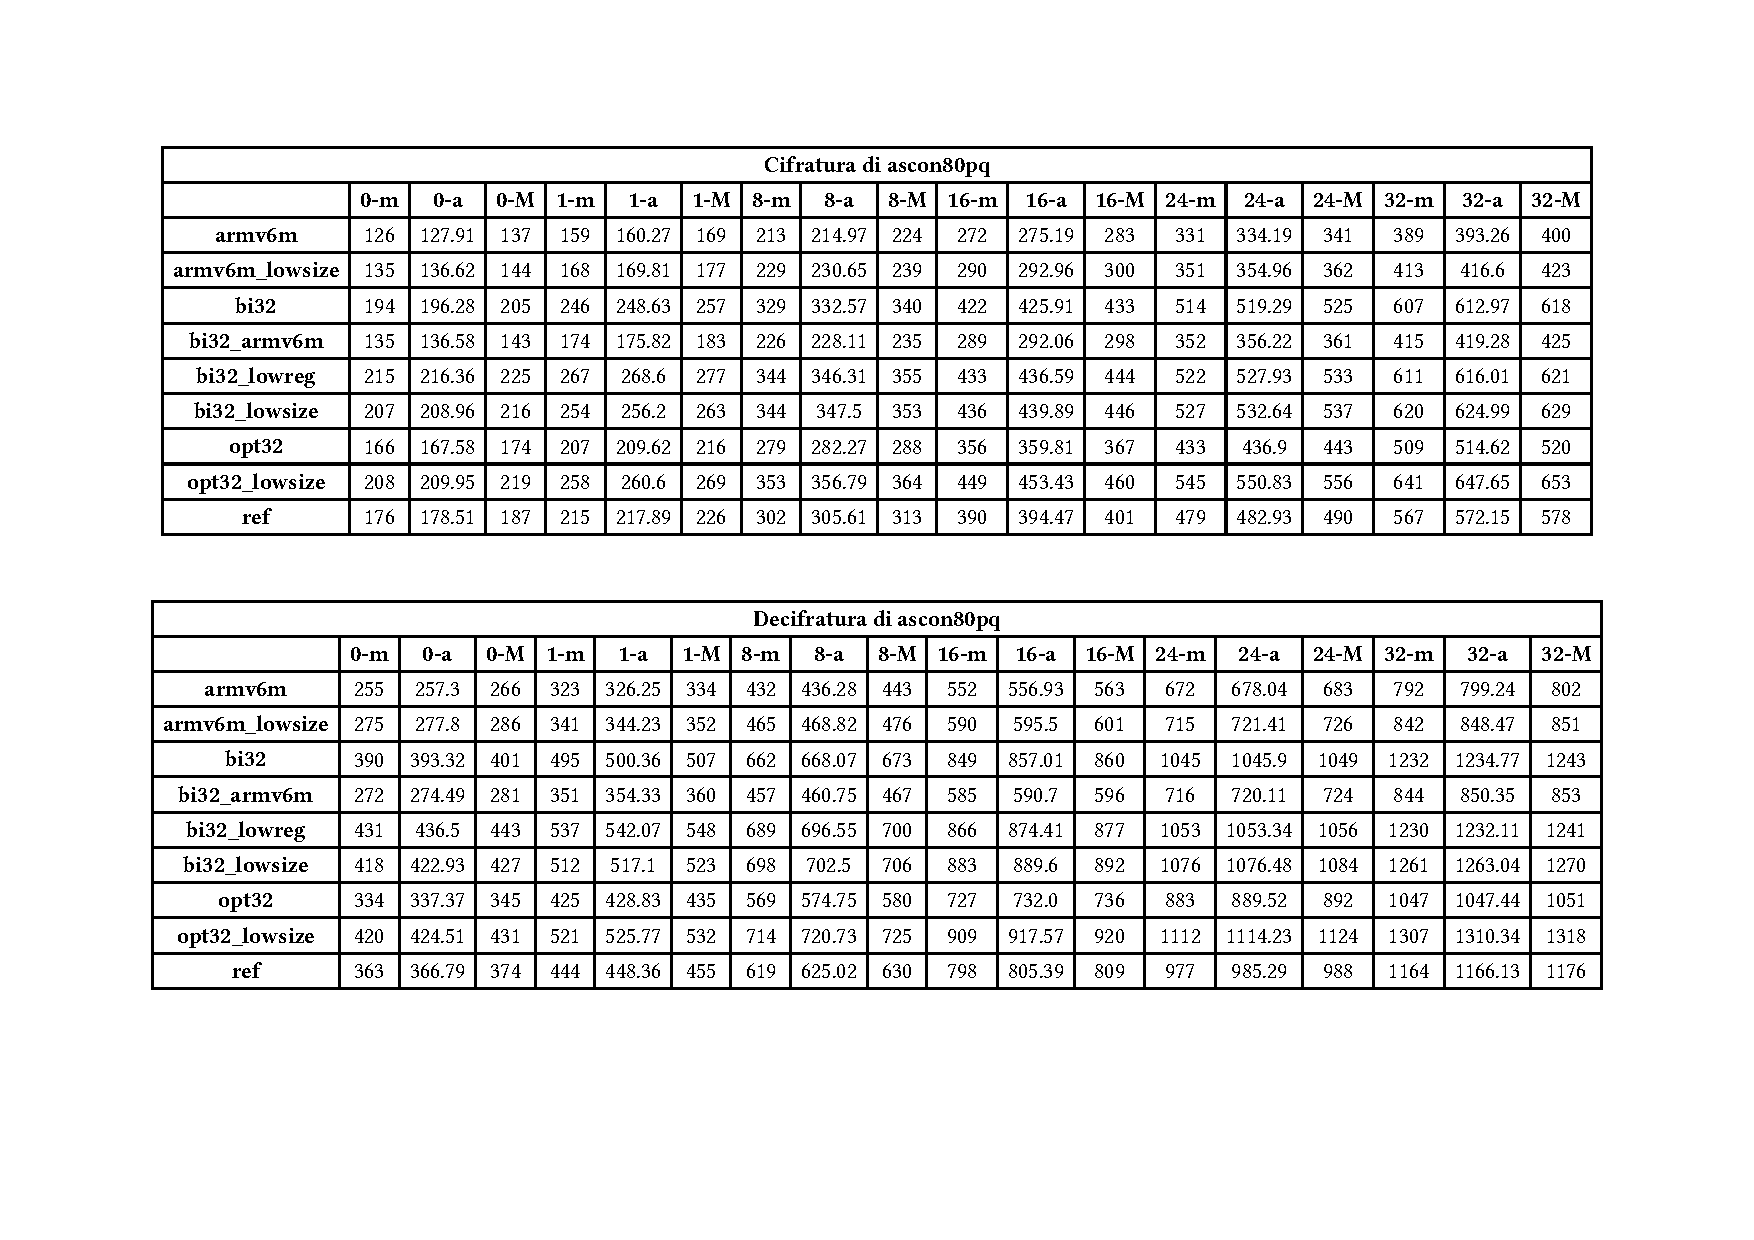
\includegraphics[width=\textwidth]{adafruit/ascon80pq.pdf}

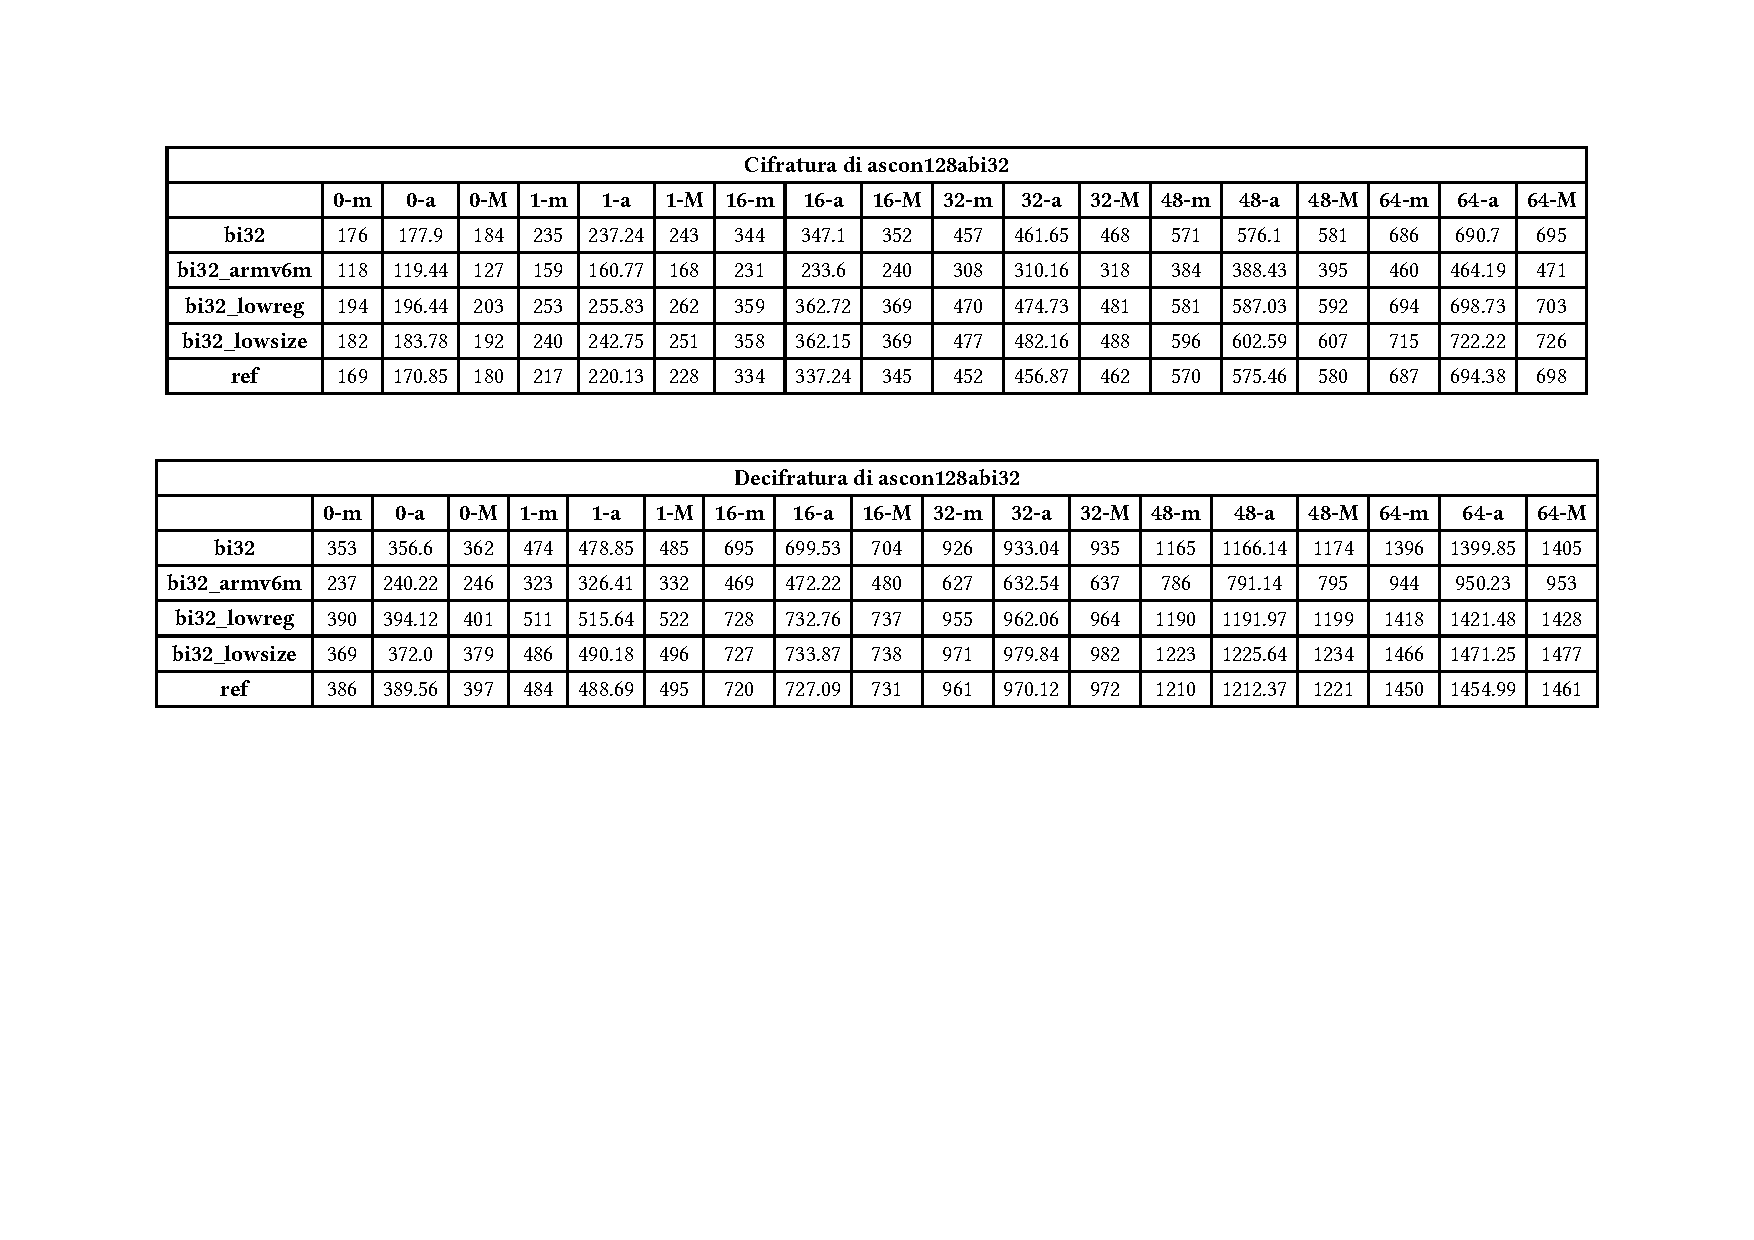
\includegraphics[width=\textwidth]{adafruit/ascon128abi32.pdf}

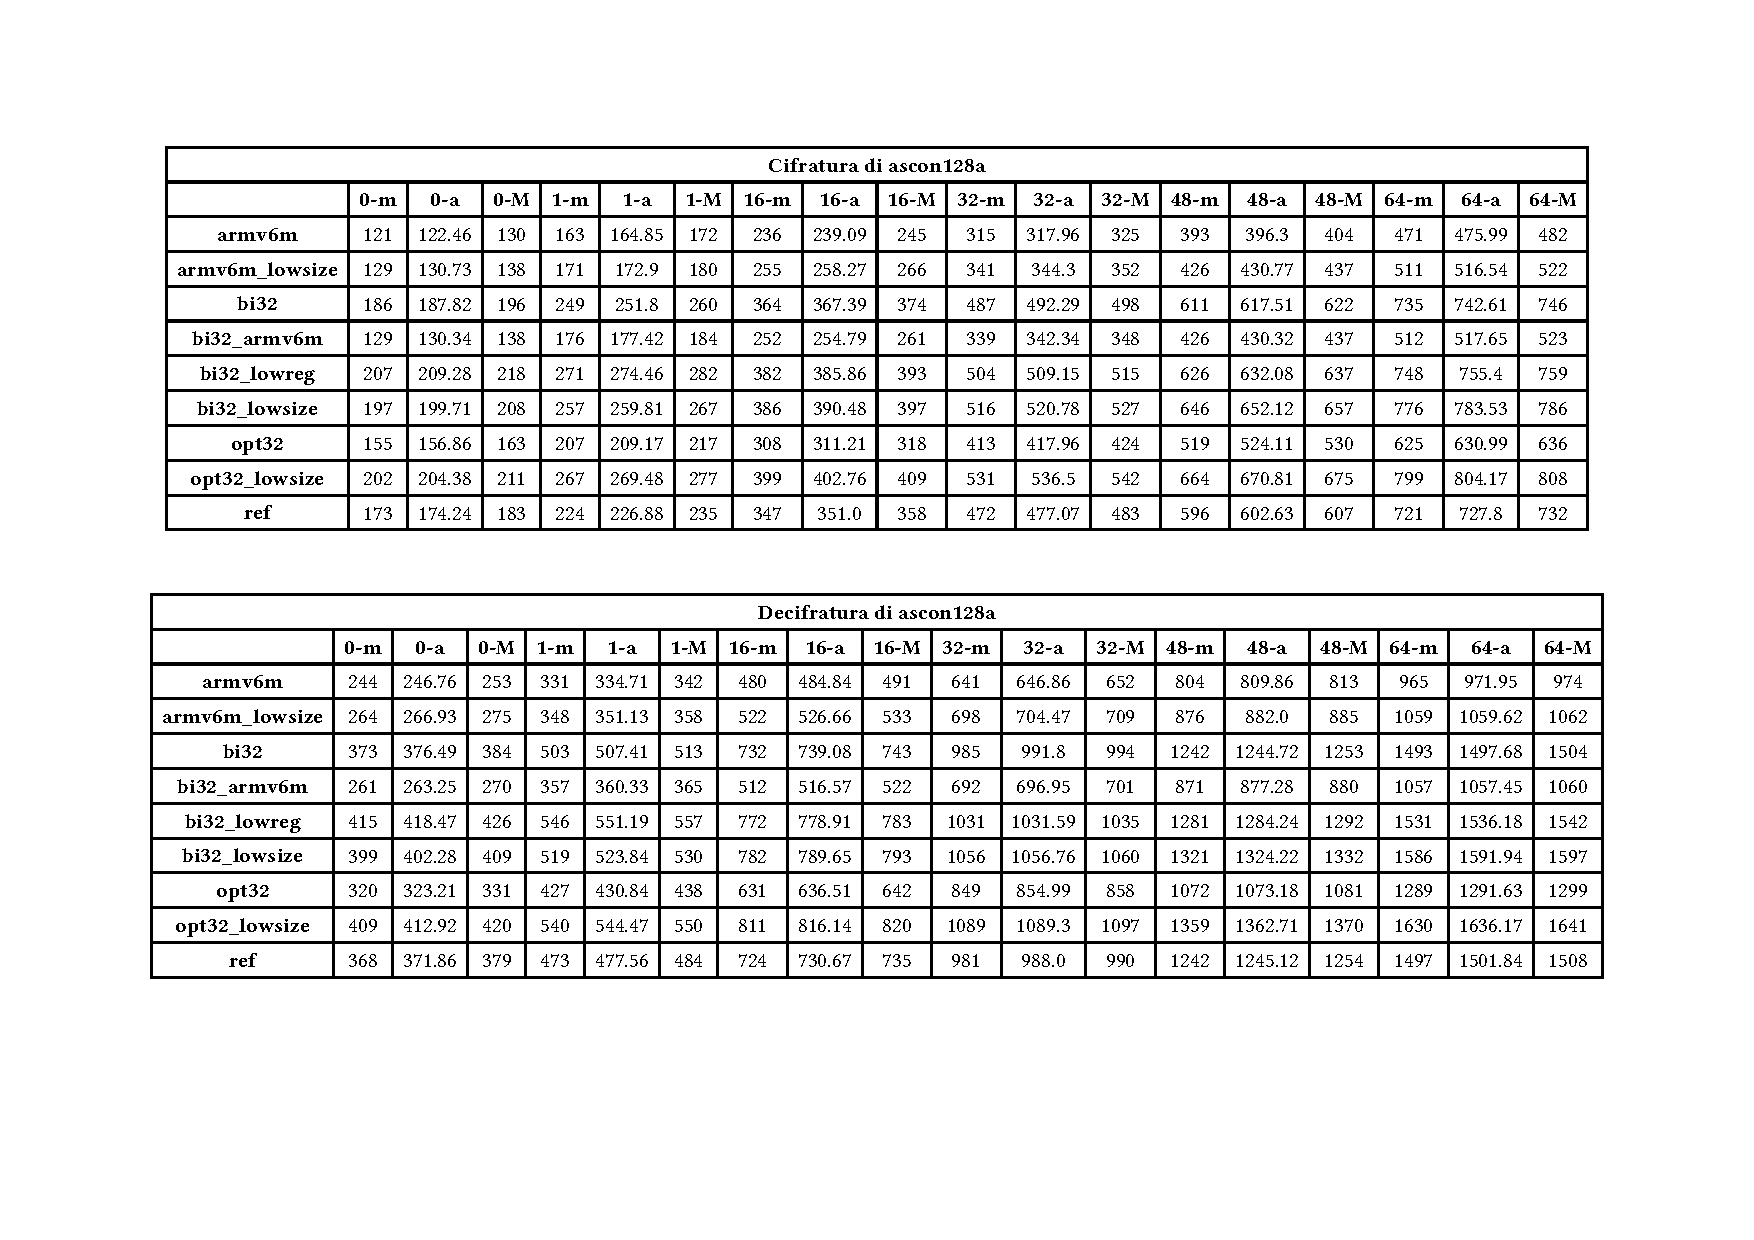
\includegraphics[width=\textwidth]{adafruit/ascon128a.pdf}

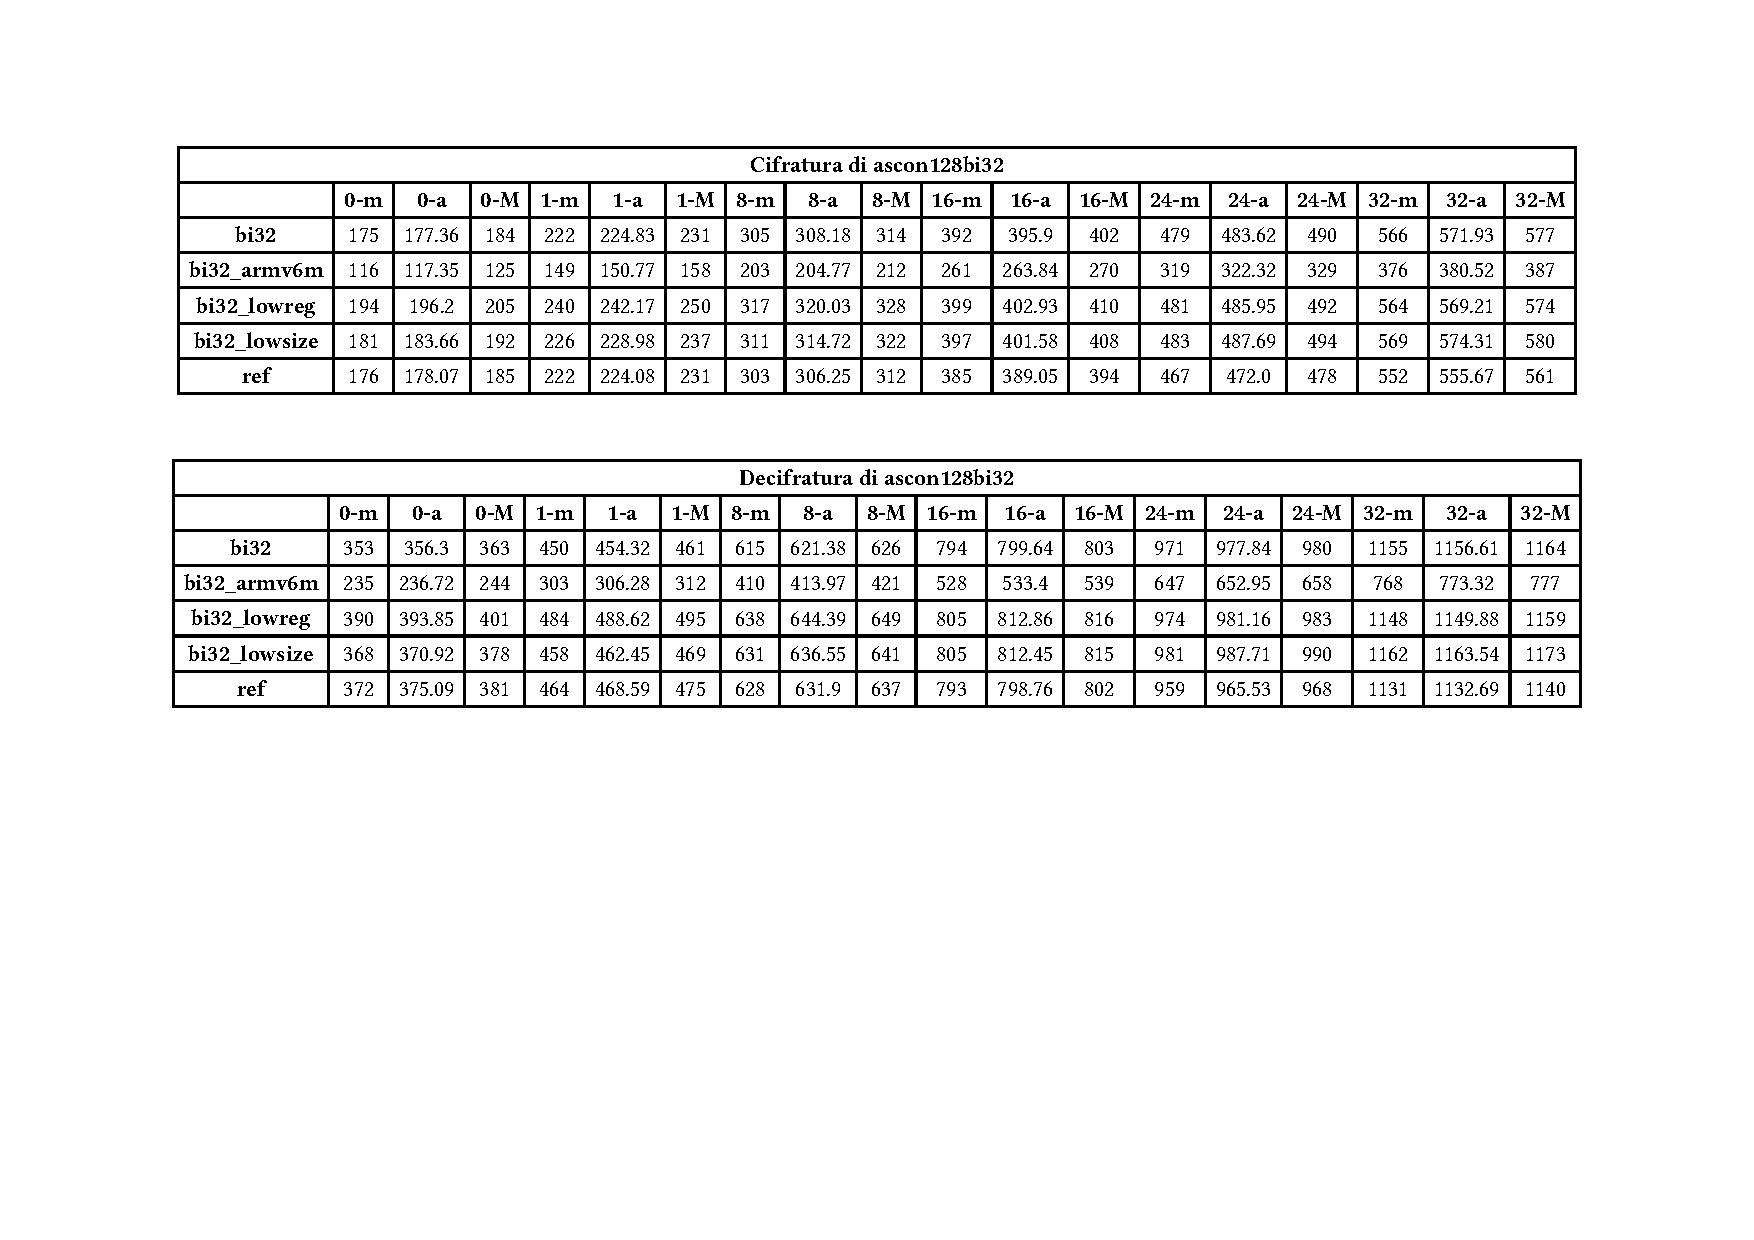
\includegraphics[width=\textwidth]{adafruit/ascon128bi32.pdf}

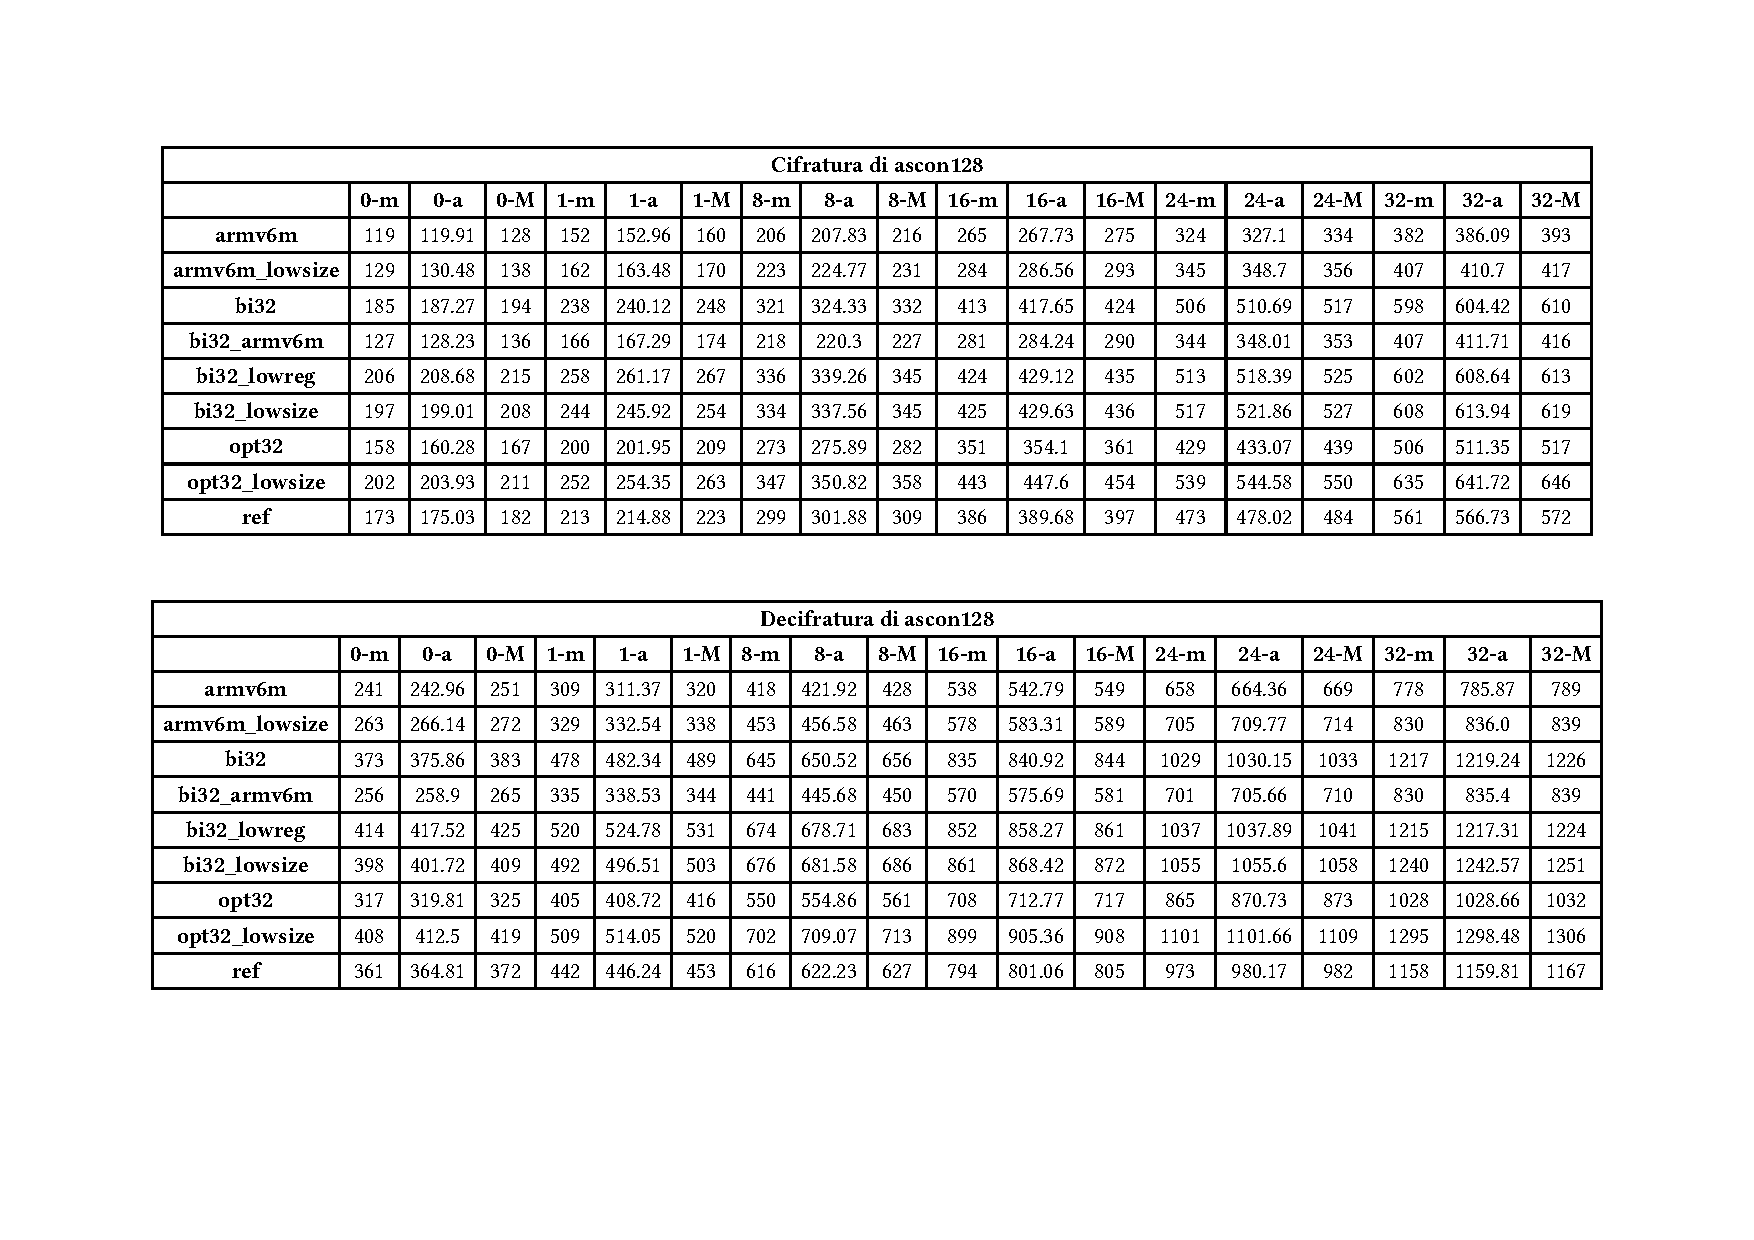
\includegraphics[width=\textwidth]{adafruit/ascon128.pdf}

% Fase di DEC

\subsubsection{Crypto hash}

Per la famiglia crypto hash sono state testate le implementazioni ARMv6-M, ARMv6-M lowsize, bi32, bi32 ARMv6-M, bi32 lowreg, bi32 lowsize, opt32, opt32 lowsize e ref.

Inserisci tabelle appena capisci come fare.

\subsubsection{Crypto auth}

Per la famiglia crypto auth sono state testate le implementazioni ARMv6-M, bi32, bi32 ARMv6-M, bi32 lowreg, opt32 e ref.

Inserisci tabelle appena capisci come fare.

\subsection{Arduino Due}

Una subsubsection per ogni famiglia con i risultati

\subsection{Raspberry qualcosa}

Una subsubsection per ogni famiglia con i risultati

\newpage

\chapter{Conclusioni}

1 pagina dove termino il discorso

\newpage

\printbibliography

\end{document}
